% Chapter "Grover" -- build with:  latexmk -pdf grover_chapter.tex
\documentclass[11pt,a4paper,openany]{book}
\usepackage[a4paper, top=22mm, bottom=22mm, left=22mm, right=22mm, headheight=14pt]{geometry}
\usepackage[T1]{fontenc}
\usepackage{lmodern}
\usepackage{amsmath, amssymb, mathtools, amsthm}
\usepackage{braket}
\usepackage{array, tabularx, booktabs}
\usepackage{enumitem}
\usepackage[dvipsnames]{xcolor}
\usepackage[most]{tcolorbox}
\usepackage{tikz}
\usetikzlibrary{arrows.meta, calc}
\usepackage{pgfplots}
\pgfplotsset{compat=1.17}
\usepackage{fancyhdr}
\usepackage[hidelinks]{hyperref}
\usepackage{needspace}

\definecolor{brand}{HTML}{1F4E79}
\definecolor{okgreen}{HTML}{1B7F3B}
\definecolor{warn}{HTML}{B5551B}
\setlength{\parindent}{0pt}
\setlength{\parskip}{5pt}
\allowdisplaybreaks

\newtcolorbox{defn}[1]{enhanced, breakable, colback=brand!5, colframe=brand, fonttitle=\bfseries, title={Definition: #1}}
\newtcolorbox{keyres}[1]{enhanced, breakable, colback=okgreen!5, colframe=okgreen!70!black, fonttitle=\bfseries, title={Key result: #1}}
\newtcolorbox{trap}{enhanced, breakable, colback=warn!6, colframe=warn, fonttitle=\bfseries, title={Common trap}}
\newtcolorbox{method}[1]{enhanced, breakable, colback=black!3, colframe=black!55, fonttitle=\bfseries, title={Method: #1}}
\newcounter{wex}[section]
\newtcolorbox{wexample}[1]{enhanced, breakable, colback=white, colframe=brand!60, coltitle=black, colbacktitle=brand!15,
  fonttitle=\bfseries, title={\refstepcounter{wex}Worked example \thesection.\arabic{wex}: #1}}
\newenvironment{keepfig}{\par\noindent\begin{minipage}{\linewidth}\centering}{\end{minipage}\par\medskip}
\newenvironment{steps}{\begin{enumerate}[label=\textbf{Step \arabic*.}, leftmargin=4.2em, itemsep=2pt]}{\end{enumerate}}

\pagestyle{fancy}\fancyhf{}
\fancyhead[L]{\small\color{black!70}Chapter: Grover}
\fancyhead[R]{\small\color{black!70}\rightmark}
\fancyfoot[C]{\small\thepage}
\renewcommand{\headrulewidth}{0.4pt}
\renewcommand{\thesection}{\arabic{section}}
\renewcommand{\sectionmark}[1]{\markright{\thesection.\ #1}}

\newcommand{\kopt}{k_{\rm opt}}
\newcommand{\xs}{x^\ast}
\newcommand{\proj}[1]{\ket{#1}\!\bra{#1}}

% =====================================================================================
% SILICO FELLER branding for the book chapters (and any other A4 document).
% \input this file in the preamble of every book/<algorithm>_chapter_source/<algorithm>_chapter.tex.
% The official logo (assets/branding/silico_feller_logo.png, unmodified, aspect ratio kept) is drawn as a
% light watermark (~8 % opacity) in the page background of EVERY page, behind all text, equations and figures -
% the same treatment as the question papers and answer books.
% =====================================================================================
\usepackage{graphicx}
\usepackage{tikz}
\usepackage{eso-pic}
\AddToShipoutPictureBG{\AtPageCenter{\makebox(0,0){\tikz\node[opacity=0.08, inner sep=0pt]{
\includegraphics[width=0.72\paperwidth]{../../assets/branding/silico_feller_logo.png}};}}}
   % SILICO FELLER watermark on every page
\begin{document}
\begin{titlepage}
\centering
{\color{brand}\rule{\linewidth}{1.5pt}}\\[10pt]
{\Huge\bfseries\color{brand} Grover}\\[8pt]
{\LARGE Grover's Search Algorithm}\\[6pt]
{\large A step-by-step chapter: from reflections in the plane to amplitude amplification}\\[6pt]
{\color{brand}\rule{\linewidth}{1.5pt}}
\vspace{18mm}

\begin{minipage}{0.86\linewidth}
\large
\textbf{What you will be able to do after this chapter}
\begin{itemize}[itemsep=3pt]
\item use the trigonometric identities and reflection matrices behind the algorithm without a calculator;
\item manipulate superpositions, signs, measurements and multi-controlled gates with confidence;
\item build the oracle and the diffusion circuit for any marked string, and count their gates;
\item trace amplitudes by hand with inversion about the mean, and explain the same steps as a rotation;
\item find the optimal number of iterations, and predict over-rotation, for one or for many solutions;
\item reason about unknown $M$, exact and fixed-point search, amplitude amplification and quantum counting;
\item solve every type of question in the accompanying 80-question Grover assessment.
\end{itemize}
\end{minipage}
\vfill
{\small Companion material in the same repository: \texttt{presentations/Grover\_Lecture.pdf} (slides),
\texttt{Grover.ipynb} (CUDA-Q notebook) and \texttt{assessments/} (question paper and answer book).}
\end{titlepage}

\tableofcontents
\setcounter{chapter}{0}
\chapter*{Grover --- Quantum Search}
\addcontentsline{toc}{chapter}{Grover --- Quantum Search}
\markboth{Grover}{Grover}

\section*{How to use this chapter}
The chapter is built as a staircase. Sections~1--3 are the \emph{mathematics} you need (trigonometry, reflections and
rotations, averages and counting). Sections~4--5 are the \emph{quantum mechanics} (states, measurement, gates, kickback).
Sections~6--11 are \emph{Grover's algorithm itself}. Sections~12--14 are the \emph{advanced} material: unknown $M$, exact
and fixed-point search, amplitude amplification, quantum counting and the limits of the speed-up. Section~15 collects
problem-solving strategies and Section~16 has practice problems with answers.

Each section has: the idea in words, the precise statement, a derivation, \textbf{worked examples} solved step by step,
\textbf{common traps} (the wrong answers examiners like to offer) and a short checklist. Do the worked examples with a
pencil before reading the solution.

\begin{defn}{Conventions used everywhere in this chapter}
\begin{itemize}[leftmargin=1.2em, itemsep=1pt]
\item $n$ qubits, $N = 2^n$ items, $M$ marked items ($M = 1$ unless stated otherwise).
\item $\ket{x} = \ket{x_1x_2\dots x_n}$ with $x = x_1 2^{n-1} + \dots + x_n 2^0$: \textbf{qubit 1 is the most significant bit}.
\item $\ket{s} = H^{\otimes n}\ket{0\dots0} = \frac{1}{\sqrt N}\sum_x\ket{x}$; oracle $U_\omega\ket{x} = (-1)^{f(x)}\ket{x}$; diffusion $D = 2\proj{s} - I$; iteration $G = DU_\omega$ (oracle first).
\item $\sin\theta = \sqrt{M/N}$, $\;P_k = \sin^2((2k+1)\theta)$, $\;\kopt = \operatorname{round}\big(\frac{\pi}{4\theta} - \frac12\big)$.
\item \textbf{Notebook naming:} \texttt{Grover.ipynb} writes \texttt{N\_QUBITS} (or $N$) for our $n$, $M = 2^N$ for our $N$, and $O$ for our $U_\omega$. It treats one marked item and prints qubit 0 first. The formulas are the same.
\end{itemize}
\end{defn}

%=====================================================================================================
\section{Complex phases and trigonometry}
\subsection{Complex numbers as phases}
A complex number $z = a + ib$ has modulus $|z| = \sqrt{a^2 + b^2}$ and polar form $z = |z|e^{i\varphi}$, where $e^{i\varphi} = \cos\varphi + i\sin\varphi$. Powers multiply the angle.
\emph{Example:} $\frac{1 - i}{\sqrt2} = e^{-i\pi/4}$, so its cube is $e^{-3i\pi/4}$. The sign flip of the oracle is the phase $-1 = e^{i\pi}$: it changes direction, never length.

\subsection{The identities you need}
Everything about the success probability follows from the angle-addition formulas:
\[ \cos2\alpha = 1 - 2\sin^2\alpha = 2\cos^2\alpha - 1, \qquad \sin2\alpha = 2\sin\alpha\cos\alpha, \qquad \sin3\alpha = 3\sin\alpha - 4\sin^3\alpha. \]
The last one, squared and written with $s = \sin^2\alpha$, is worth remembering:
\begin{keyres}{Probability after one iteration}
\[ \sin^2 3\alpha = s(3 - 4s)^2, \qquad s = \sin^2\alpha. \]
\end{keyres}

\begin{wexample}{An exact value}
Let $\sin\theta = \frac13$. Find $\sin^2 3\theta$ and $\cos2\theta$.
\begin{steps}
\item $\sin3\theta = 3\cdot\frac13 - 4\cdot\frac{1}{27} = 1 - \frac{4}{27} = \frac{23}{27}$, so $\sin^2 3\theta = \frac{529}{729}$.
\item $\cos2\theta = 1 - 2\cdot\frac19 = \frac79$.
\end{steps}
\textbf{Check} with the boxed form: $s = \frac19$ gives $\frac19\big(3 - \frac49\big)^2 = \frac19\cdot\frac{529}{81} = \frac{529}{729}$. \checkmark
\end{wexample}

\subsection{Small angles}
For small $x$: $\sin x \approx x$ and $\arcsin x = x + \frac{x^3}{6} + \dots$. So $\arcsin x$ is slightly \emph{larger} than $x$ for $x > 0$.
Example: $\arcsin 0.125 = 0.12533$. This is why $\theta \approx 1/\sqrt N$ is good for large $N$ but not exact.

\subsection{The curve $\sin^2((2k+1)\theta)$}
The function $\sin^2$ has period $\pi$ (not $2\pi$) and equals $1$ at odd multiples of $\frac\pi2$. Moving from $k$ to $k + p$ adds $2p\theta$ to the angle.
\begin{keyres}{Peak and period}
$\sin^2((2k+1)\theta) = 1$ needs $(2k+1)\theta$ to be an odd multiple of $\frac\pi2$. The sequence repeats with period $p$ whenever $2p\theta$ is a multiple of $\pi$; the
natural period is $\frac{\pi}{2\theta}$ iterations when this is an integer.
\end{keyres}

\begin{wexample}{First maximum, period and window}
Let $\theta = \frac{\pi}{14}$.
\begin{steps}
\item First maximum: $(2k+1)\frac{\pi}{14} = \frac\pi2$ gives $2k + 1 = 7$, so $k = 3$.
\item Period: $2p\frac{\pi}{14} = m\pi$ gives $p = 7m$, so the smallest period is $7$.
\item Window $P \ge \frac34$: the angle must be within $\frac\pi6$ of $\frac\pi2$, i.e.\ $\frac{\pi}{3} \le (2k+1)\frac{\pi}{14} \le \frac{2\pi}{3}$, so $4.67 \le 2k + 1 \le 9.33$: $2k + 1 \in \{5, 7, 9\}$, or $k = 2, 3, 4$.
\end{steps}
\end{wexample}

\textbf{Checklist 1.} Square at the end; period of $\sin^2$ is $\pi$; use degrees if it makes the list of angles easier to read; check with $s(3 - 4s)^2$.

%=====================================================================================================
\section{Reflections and rotations}
\subsection{Reflection matrices}
\begin{defn}{Reflection about a unit vector}
For a unit vector $\ket{u}$, the operator $R_u = 2\proj{u} - I$ fixes $\ket{u}$ and negates every vector orthogonal to $\ket{u}$.
\end{defn}
Because $\braket{u|u} = 1$, expanding gives $R_u^2 = 4\ket{u}\braket{u|u}\bra{u} - 4\proj{u} + I = I$. So a reflection is its own inverse; it is Hermitian, and hence unitary.
\begin{keyres}{Spectrum and trace in dimension $N$}
$R_u$ has eigenvalue $+1$ once and $-1$ exactly $N - 1$ times, so $\operatorname{tr} R_u = 2 - N$. The projector $\proj{u}$ has trace $1$ and is \emph{not} unitary.
\end{keyres}

\begin{wexample}{A $2\times2$ reflection}
Let $u = (\frac{5}{13}, \frac{12}{13})^{T}$.
\begin{steps}
\item $uu^{T} = \frac{1}{169}\begin{psmallmatrix}25&60\\60&144\end{psmallmatrix}$, so $2uu^{T} - I = \frac{1}{169}\begin{psmallmatrix}50 - 169 & 120\\ 120 & 288 - 169\end{psmallmatrix} = \frac{1}{169}\begin{psmallmatrix}-119 & 120\\ 120 & 119\end{psmallmatrix}$.
\item Check that it fixes $u$: first entry $\frac{1}{169\cdot13}(-119\cdot5 + 120\cdot12) = \frac{845}{2197} = \frac{5}{13}$. \checkmark\ Trace $0$, determinant $-1$.
\end{steps}
\end{wexample}

\subsection{Two reflections make a rotation}
In the plane, a reflection in the line at angle $\alpha$ sends a vector at angle $\phi$ to angle $2\alpha - \phi$.
\begin{keyres}{Composition}
Reflecting in the line at $\alpha$ and then in the line at $\beta$ gives $\phi \mapsto 2\beta - (2\alpha - \phi) = \phi + 2(\beta - \alpha)$: a \textbf{rotation by twice the angle between the lines}, directed from the first line to the second.
\end{keyres}
\begin{wexample}{Order matters}
Lines at $20^\circ$ and $50^\circ$. First $20^\circ$, then $50^\circ$: rotation by $+60^\circ$. In the opposite order: rotation by $-60^\circ$. The product of two reflections has determinant $(-1)(-1) = +1$, so it can never be a reflection.
\end{wexample}

\subsection{Eigenvalues and powers of a rotation}
$R(\alpha) = \begin{psmallmatrix}\cos\alpha & -\sin\alpha\\ \sin\alpha & \cos\alpha\end{psmallmatrix}$ has eigenvalues $e^{\pm i\alpha}$ with eigenvectors $\frac{1}{\sqrt2}(1, \mp i)^{T}$, and powers simply add angles: $R(\alpha)^k = R(k\alpha)$.
\begin{wexample}{Eigenvalues and a power}
\begin{steps}
\item Let $\alpha = 2\theta$ with $\sin\theta = \frac13$. Then $\cos2\theta = \frac79$ and $\sin2\theta = 2\cdot\frac13\cdot\frac{2\sqrt2}{3} = \frac{4\sqrt2}{9}$. Eigenvalues: $\frac{7 \pm 4\sqrt2\,i}{9}$; modulus $\sqrt{49 + 32}/9 = 1$. \checkmark
\item The rotation by $45^\circ$ satisfies $R^k = -I$ first at $k = 4$, and $R^k = +I$ first at $k = 8$.
\end{steps}
\end{wexample}

\begin{trap}
Eigenvalues of a rotation by $2\theta$ involve $2\theta$, not $\theta$. Real numbers $\pm1$ occur only for rotations by $0$ or $\pi$ --- and for reflections.
\end{trap}

\textbf{Checklist 2.} Test a reflection by what it fixes; determinant $-1$ (plane) tells reflection from rotation; rotation angle is twice the angle between the lines.

%=====================================================================================================
\section{Averages, counting and classical search}
\subsection{Inversion about the mean}
\begin{defn}{Inversion about the mean}
For a list $v_1, \dots, v_N$ with mean $\bar v$: $\;v_j \mapsto 2\bar v - v_j$. Every entry is reflected through the mean: a distance $d$ below becomes a distance $d$ above.
\end{defn}
The mean is unchanged and the sum of squares is preserved (Section~7 shows why this is unitary).
\begin{wexample}{Sixteen entries}
$v$ has $15$ entries $+1$ and one entry $-1$. The mean is $\frac{14}{16} = \frac78$. The special entry becomes $\frac74 + 1 = \frac{11}{4}$; the others become $\frac74 - 1 = \frac34$.
Length check: $15\cdot\frac{9}{16} + \frac{121}{16} = \frac{256}{16} = 16$. \checkmark
\end{wexample}

\subsection{Counting solutions}
The quantity that controls Grover's algorithm is the \textbf{fraction of solutions} $M/N$. If the conditions involve disjoint groups of variables, the counts multiply.
A useful consequence of the count: $\sum_x(-1)^{f(x)} = (N - M) - M = N - 2M$.
\begin{wexample}{A small Boolean function}
$f = (x_1 \land x_2) \lor x_3$ on three bits. If $x_3 = 1$: all $4$ choices of $x_1x_2$ work. If $x_3 = 0$: only $x_1x_2 = 11$. So $M = 5$, $M/N = \frac58$, and $\sum_x(-1)^{f(x)} = 8 - 10 = -2$.
\end{wexample}

\subsection{Classical search}
\textbf{Structure decides the cost.} On a \emph{sorted} list, binary search halves the range at each step, so $2^{b} - 1$ entries take at most $b$ comparisons. On an \emph{unsorted} list, a key that may be absent needs up to $N$ comparisons. \emph{Example:} $N = 255$: at most $8$ and $255$. Grover's algorithm concerns the unsorted case.

\begin{keyres}{Expected number of queries}
Drawing \textbf{without} replacement: $\dfrac{N + 1}{M + 1}$. (The $M$ marked items split the $N - M$ others into $M + 1$ gaps of equal mean size.) \\[2pt]
Drawing \textbf{with} replacement: $\dfrac{N}{M}$ (geometric distribution). \\[2pt]
For one marked item: $\frac{N+1}{2}$ without replacement. The classical cost is $\Theta(N/M)$.
\end{keyres}
\textbf{At least one success.} $r$ independent runs with success probability $p$ succeed at least once with probability $1 - (1-p)^r$. Example: $p = \frac12$, $r = 4$: $\frac{15}{16}$.

\subsection{Square-root scaling}
$\sqrt{N} = 2^{n/2}$, so each extra qubit multiplies $\sqrt N$ by $\sqrt2$. Adding $4$ bits multiplies the search space by $16$ and $\sqrt N$ by $4$.

\textbf{Checklist 3.} Mean first, then invert; check length; ``at least one'' means use the complement; with or without replacement gives different formulas.

%=====================================================================================================
\section{Qubits, states and measurement}
\subsection{States and the Born rule}
$\ket\psi = \sum_x c_x\ket{x}$ with $\sum_x|c_x|^2 = 1$. \textbf{Born rule:} measuring all qubits gives $x$ with probability $|c_x|^2$. The uniform state $\ket{s}$ has every $c_x = 1/\sqrt N$ and is a product of $\ket{+}$ states, so its qubits are independent.
\emph{Example:} in $H^{\otimes4}\ket{0000}$, $P(x_1 = 0, x_4 = 1) = \frac{4}{16} = \frac14$.

\begin{method}{Measuring only a property (subspace measurement)}
(1) Group the basis states that have the property. (2) The probability is the sum of $|c_x|^2$ over the group. (3) The new state is that group alone, \emph{re-normalised}; it stays a superposition.
\end{method}
\begin{wexample}{Grover's final step in miniature}
$\ket\psi = \frac13(2\ket{00} + \ket{01} + \ket{10} + \sqrt3\ket{11})$. Ask ``are the two bits equal?''
\begin{steps}
\item The group is $\{\ket{00}, \ket{11}\}$. $P = \frac{4 + 3}{9} = \frac79$.
\item New state: $\frac{2\ket{00} + \sqrt3\ket{11}}{\sqrt7}$.
\end{steps}
\end{wexample}

\subsection{Global versus relative phase}
\begin{keyres}{Phases}
$e^{i\gamma}\ket\psi$ and $\ket\psi$ are \textbf{the same physical state}. A sign on \emph{one} amplitude of a superposition is a \textbf{relative} phase. It does not change computational-basis probabilities, but it does change results after an interfering gate such as $H$.
\end{keyres}
This single distinction explains both why the oracle alone gives nothing (Section~6) and why the $-1$ in the diffusion circuit is harmless (Section~10).

\subsection{Normalisation and tensor products}
Every term in the normalisation condition is a squared \emph{modulus}: $\;|a + ib|^2 = a^2 + b^2$. \emph{Example:} $c(\ket0 + (1 - i)\ket1)$ needs $c^2(1 + 2) = 1$, so $c = \frac{1}{\sqrt3}$.
For two independent qubits, $(a_0\ket0 + a_1\ket1)\otimes(b_0\ket0 + b_1\ket1)$ has the amplitude $a_jb_k$ on $\ket{jk}$. \emph{Example:} $\frac{1}{\sqrt2}(\ket0 - i\ket1)\otimes\frac{1}{\sqrt2}(\ket0 + \ket1)$ has $-\frac i2$ on $\ket{11}$.

\subsection{Overlaps}
$\braket{a|b} = \sum_x\overline{a_x}b_x$ (conjugate the \emph{first} vector), and $|\braket{a|b}|^2$ is a probability. \emph{Example:} for $a = \frac{1}{\sqrt2}(1, i)$, $b = (1, 0)$: $\;\braket{a|b} = \frac{1}{\sqrt2}$; for $a = \frac{1}{\sqrt2}(1, i)$, $b = (0, 1)$: $\;\braket{a|b} = -\frac{i}{\sqrt2}$. If $\ket{r}$ is the uniform superposition of the $N - 1$ unmarked items, then
$\braket{r|s} = (N - 1)\frac{1}{\sqrt{N-1}\sqrt N} = \sqrt{\frac{N-1}{N}}$. For $N = 8$: $\sqrt{7/8}$.

\subsection{Memory of a state-vector simulation}
$2^n$ amplitudes $\times$ bytes per amplitude: $16$ B in double precision (\texttt{fp64}), $8$ B in single (\texttt{fp32}). $n = 28$ in double: $4$ GiB; $n = 31$: $32$ GiB. The notebook's iteration sweep holds two states at once and therefore needs twice this.

%=====================================================================================================
\section{Gates for Grover}
\subsection{Hadamard layers}
$H\ket0 = \ket{+}$, $H\ket1 = \ket{-}$, and $H^{\otimes n}\ket{x} = \frac{1}{\sqrt N}\sum_y(-1)^{x\cdot y}\ket{y}$ with $x\cdot y = \sum_j x_jy_j$. \emph{Example:} in $H^{\otimes3}\ket{101}$ the amplitude of $\ket{110}$ has $x\cdot y = 1 + 0 + 0 = 1$, so it is $-\frac{1}{\sqrt8}$.

\begin{center}
\renewcommand{\arraystretch}{1.25}
\begin{tabular}{@{}l|cccc@{}}
\toprule
 & $\ket0$ & $\ket1$ & $\ket{+}$ & $\ket{-}$\\ \midrule
$H$ & $\ket{+}$ & $\ket{-}$ & $\ket0$ & $\ket1$\\
$X$ & $\ket1$ & $\ket0$ & $\ket{+}$ & $-\ket{-}$\\
$Z$ & $\ket0$ & $-\ket1$ & $\ket{-}$ & $\ket{+}$\\
\bottomrule
\end{tabular}
\end{center}
Also $HXH = Z$, $HZH = X$. For one qubit, $2\proj{+} - I = X$ and $2\proj{0} - I = Z$.

\subsection{Multi-controlled gates}
The multi-controlled $Z$ (written C$^{n-1}$Z, or CCZ for three qubits) is $\operatorname{diag}(1, \dots, 1, -1) = I - 2\proj{1\dots1}$. It is symmetric: every qubit can be regarded as the target. Hadamards on the target turn a multi-controlled $X$ into a multi-controlled $Z$, as in $(I \otimes I \otimes H)\,\mathrm{CCX}\,(I \otimes I \otimes H) = \mathrm{CCZ}$.

\begin{keyres}{Moving the sign flip with $X$ gates}
Conjugating by $X$ on selected qubits moves the affected basis state: if $X_S$ maps $\ket{a}$ to $\ket{1\dots1}$, then $X_S\,\mathrm{C}^{n-1}\mathrm{Z}\,X_S = I - 2\proj{a}$.
\end{keyres}
\begin{wexample}{Selecting a basis state}
To flip the sign of $\ket{110}$ on three qubits: apply $X$ to qubit 3 (the only $0$), then CCZ, then $X$ on qubit 3 again. Only $\ket{110}$ is mapped to $\ket{111}$, and only it picks up the sign.
\end{wexample}

\subsection{Phase kickback}
\begin{keyres}{Bit oracle to phase oracle}
For $U_f\ket{x}\ket{y} = \ket{x}\ket{y \oplus f(x)}$: \quad $U_f\ket{x}\ket{-} = (-1)^{f(x)}\ket{x}\ket{-}$, \quad but \quad $U_f\ket{x}\ket{+} = \ket{x}\ket{+}$.
\end{keyres}
\emph{Reason:} $\ket{\pm}$ are eigenvectors of $X$ with eigenvalues $\pm1$; if $f(x) = 1$ the ancilla receives an $X$. The ancilla stays in a product with the input register, so it can be measured or re-used without disturbing anything.

\begin{wexample}{Toffoli as a two-qubit phase oracle}
Start with $\ket{00}\ket{1}$ and apply $H$ to all three, then Toffoli. With $f = x_1 \land x_2$: state $= \frac12(\ket{00} + \ket{01} + \ket{10} - \ket{11})\ket{-}$. Measuring the ancilla gives $0$ or $1$ with probability $\frac12$ each and leaves the first factor unchanged.
\end{wexample}

\subsection{Entanglement test}
\begin{keyres}{Product test for two qubits}
$\sum c_{jk}\ket{jk}$ is a product state $\iff c_{00}c_{11} = c_{01}c_{10}$.
\end{keyres}
Examples: $\frac12(1, -1, 1, -1)$: $-\frac14 = -\frac14$, product $\ket{+}\ket{-}$. $\;\frac12(1, 1, -1, 1)$: $\frac14 \ne -\frac14$, entangled. So a single sign flip on $\ket{s}$ with $n = 2$ produces entanglement.

\begin{trap}
$Z \otimes Z \otimes Z$ is not CCZ: it flips the sign of every odd-weight string. And $\ket{-}$, not $\ket{+}$, is the ancilla that gives kickback.
\end{trap}

%=====================================================================================================
\section{The search problem and the oracle}
\begin{defn}{Unstructured search}
Given a black box for $f: \{0,1\}^n \to \{0,1\}$ with $f(x) = 1$ exactly on the $M$ marked items, find one marked item using as few queries as possible.
\end{defn}
The oracle does not ``know the answer'' in a useful way: it only recognises a solution, as a program checks a candidate. For $M = 1$:
\[ U_\omega = I - 2\proj{\xs}. \]
\begin{keyres}{The oracle alone reveals nothing}
$U_\omega$ only changes signs. On $\ket{s}$ it leaves every magnitude at $1/\sqrt N$, so a measurement straight after the oracle is uniformly random.
\end{keyres}
\begin{keyres}{The marked item does not matter}
Only $\braket{\xs|s} = 1/\sqrt N$ enters the analysis, and it is the same for every $\xs$. This symmetry of $\ket{s}$ --- not the fact that $U_\omega$ is diagonal --- is why $P_k$ is independent of the choice of $\xs$.
\end{keyres}

%=====================================================================================================
\section{Diffusion: inversion about the mean}
\begin{defn}{Diffusion operator}
$D = 2\proj{s} - I$. Since $\braket{s|\psi} = \frac{1}{\sqrt N}\sum_x c_x = \sqrt N\,\bar c$, the action on amplitudes is
\[ c_x \longmapsto 2\bar c - c_x. \]
\end{defn}
Its matrix has diagonal entries $\frac2N - 1$ and off-diagonal entries $\frac2N$, because every entry of $\proj{s}$ is $\frac1N$. For $N = 8$ these are $-\frac34$ and $\frac14$.
So $D$ is exactly inversion about the mean, and it is unitary because it is a reflection. Also $D\ket{s} = \ket{s}$: if nothing is marked, nothing changes.

\begin{method}{Tracing amplitudes by hand}
(1) Oracle: change the sign of the marked amplitudes. (2) Compute the mean of \emph{all} $N$ amplitudes. (3) Replace each $c_x$ by $2\bar c - c_x$. (4) Check $\sum|c_x|^2 = 1$.
\end{method}

\begin{keepfig}
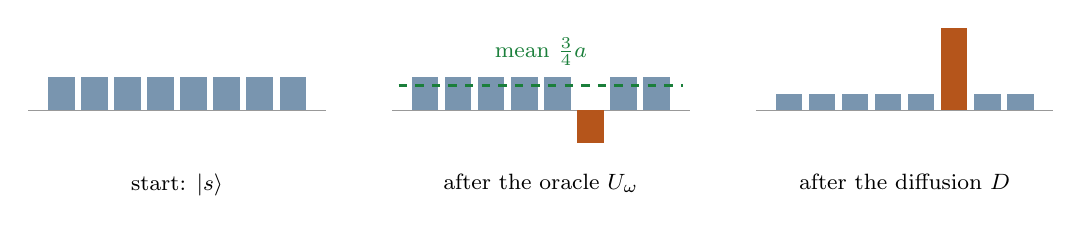
\begin{tikzpicture}[x=0.42cm, y=1.05cm]
  \foreach \offs/\lab in {0/{start: $\ket{s}$}, 11/{after the oracle $U_\omega$}, 22/{after the diffusion $D$}} {
    \draw[black!40] (\offs,0) -- (\offs+9,0);
    \node[font=\footnotesize, below] at (\offs+4.5,-0.65) {\lab};
  }
  % N = 8, amplitudes in units of a = 1/sqrt(8)
  \foreach \i in {0,...,7} {
    \fill[brand!60] (\i+0.6,0) rectangle (\i+1.4,0.4);
    \ifnum\i=5 \fill[warn] (11+\i+0.6,0) rectangle (11+\i+1.4,-0.4);
    \else \fill[brand!60] (11+\i+0.6,0) rectangle (11+\i+1.4,0.4); \fi
    \ifnum\i=5 \fill[warn] (22+\i+0.6,0) rectangle (22+\i+1.4,1.0);
    \else \fill[brand!60] (22+\i+0.6,0) rectangle (22+\i+1.4,0.2); \fi
  }
  \draw[dashed, okgreen, thick] (11.2,0.3) -- (19.8,0.3);
  \node[font=\footnotesize, okgreen, above] at (15.5,0.42) {mean $\frac34a$};
\end{tikzpicture}\\
{\small One iteration for $N = 8$, $\ket{\xs} = \ket{101}$, $a = 1/\sqrt8$: amplitudes $a \to \pm a \to (\frac12a,\ \frac52a)$.}
\end{keepfig}

\begin{wexample}{The smallest case, $N = 4$}
Amplitudes $(\frac12, \frac12, \frac12, \frac12)$. Oracle on the last: $(\frac12, \frac12, \frac12, -\frac12)$; mean $\frac14$. Inversion: $(0, 0, 0, 1)$. One iteration finds the item with \textbf{certainty}.
\end{wexample}

\begin{wexample}{Two iterations for $N = 32$}
Let $a = 1/\sqrt{32}$.
\begin{steps}
\item Oracle: mean $= \frac{30}{32}a = \frac{15}{16}a$. Marked: $\frac{15}{8}a + a = \frac{23}{8}a$. Unmarked: $\frac{15}{8}a - a = \frac78a$. $\;P_1 = \frac{529}{64}a^2 = \frac{529}{2048} \approx 0.258$.
\item Oracle again: marked $-\frac{23}{8}a$. Mean $= \frac{31\cdot\frac78 - \frac{23}{8}}{32}a = \frac{194}{256}a = \frac{97}{128}a$. Marked: $\frac{97}{64}a + \frac{184}{64}a = \frac{281}{64}a$. $\;P_2 = \frac{281^2}{64^2\cdot32} \approx 0.602$.
\end{steps}
\textbf{Check:} $\theta = 0.17771$: $\sin^2 3\theta = 0.258$ and $\sin^2 5\theta = 0.602$. \checkmark
\end{wexample}

\begin{trap}
Compute the mean \emph{after} the oracle, and include the marked item. Using the mean $a$ of the starting state, or leaving the marked item out, gives wrong numbers that look plausible. Also do not stop at the amplitude: the probability is its square.
\end{trap}

%=====================================================================================================
\section{The geometric picture}
Let $\ket{m}$ be the uniform superposition of the marked items and $\ket{r}$ that of the unmarked items. They are orthonormal and
\[ \ket{s} = \cos\theta\,\ket{r} + \sin\theta\,\ket{m}, \qquad \sin\theta = \sqrt{M/N}. \]
Both $O$ and $D$ map this plane to itself, so the whole algorithm takes place in two dimensions --- however large $N$ is.

\begin{keepfig}
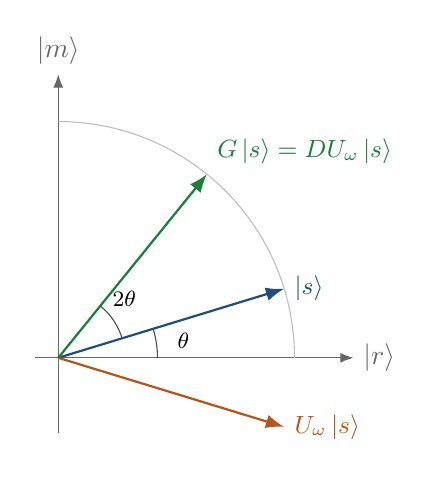
\begin{tikzpicture}[scale=3.0, >=Latex]
  \draw[->, black!60] (-0.1,0) -- (1.25,0) node[right] {$\ket{r}$};
  \draw[->, black!60] (0,-0.32) -- (0,1.2) node[above] {$\ket{m}$};
  \draw[black!25] (1,0) arc (0:90:1);
  \draw[->, thick, brand] (0,0) -- ({cos(17)},{sin(17)}) node[right, font=\small] {$\ket{s}$};
  \draw[->, thick, warn] (0,0) -- ({cos(17)},{-sin(17)}) node[right, font=\small] {$U_\omega\ket{s}$};
  \draw[->, thick, okgreen] (0,0) -- ({cos(51)},{sin(51)}) node[above right, font=\small] {$G\ket{s} = DU_\omega\ket{s}$};
  \draw[black!70] (0.42,0) arc (0:17:0.42);
  \node[font=\footnotesize] at (0.53,0.07) {$\theta$};
  \draw[black!70] (0.27,0.083) arc (17:51:0.283);
  \node[font=\footnotesize] at (0.28,0.25) {$2\theta$};
\end{tikzpicture}\\
{\small $U_\omega$ reflects in the axis $\ket{r}$; $D$ reflects in the line through $\ket{s}$; together they rotate by $2\theta$ towards $\ket{m}$.}
\end{keepfig}

\begin{steps}
\item $U_\omega$ negates $\ket{m}$ and fixes $\ket{r}$: it is the \textbf{reflection in the line through $\ket{r}$} (angle $0$).
\item $D$ fixes $\ket{s}$ and negates the perpendicular direction: it is the \textbf{reflection in the line through $\ket{s}$} (angle $\theta$).
\item By Section~2, reflecting first at angle $0$ and then at angle $\theta$ is a \textbf{rotation by $2\theta$}.
\item $\ket{s}$ starts at angle $\theta$ from $\ket{r}$, so after $k$ iterations the angle is $(2k+1)\theta$.
\end{steps}
\begin{keyres}{The state after $k$ iterations}
\[ G^k\ket{s} = \sin\big((2k+1)\theta\big)\ket{m} + \cos\big((2k+1)\theta\big)\ket{r}, \qquad P_k = \sin^2\big((2k+1)\theta\big). \]
In the basis $\{\ket{r}, \ket{m}\}$: $\;G = \begin{psmallmatrix}\cos2\theta & -\sin2\theta\\ \sin2\theta & \cos2\theta\end{psmallmatrix}$.
\end{keyres}

%=====================================================================================================
\section{Success probability and the optimal number of iterations}
We want $(2k+1)\theta$ as close as possible to $\frac\pi2$:
\begin{keyres}{Optimal number of iterations}
\[ \kopt = \operatorname{round}\Big(\frac{\pi}{4\theta} - \frac12\Big) \approx \frac\pi4\sqrt{\frac NM}, \qquad P_{\kopt} \ge 1 - \sin^2\theta = 1 - \frac MN. \]
\emph{Bound:} rounding leaves $(2k+1)\theta$ within $\theta$ of $\frac\pi2$, and $\sin^2(\frac\pi2 \pm \theta) = \cos^2\theta$.
\end{keyres}

\begin{center}
\renewcommand{\arraystretch}{1.15}
\begin{tabular}{@{}rrrrr@{}}
\toprule
$n$ & $N$ & $\theta$ (rad) & $\kopt$ & $P$\\ \midrule
$2$ & $4$ & $0.5236$ & $1$ & $1.0000$\\
$3$ & $8$ & $0.3614$ & $2$ & $0.9453$\\
$4$ & $16$ & $0.2527$ & $3$ & $0.9613$\\
$5$ & $32$ & $0.1777$ & $4$ & $0.9992$\\
$6$ & $64$ & $0.1253$ & $6$ & $0.9966$\\
$8$ & $256$ & $0.0625$ & $12$ & $0.9999$\\
$10$ & $1024$ & $0.0313$ & $25$ & $0.9995$\\
$15$ & $32\,768$ & $0.0055$ & $142$ & $1.0000$\\
$20$ & $1\,048\,576$ & $0.00098$ & $804$ & $1.0000$\\
\bottomrule
\end{tabular}
\end{center}

\begin{wexample}{Why $-\frac12$ matters: $n = 8$}
\begin{steps}
\item Rule of thumb: $\frac\pi4\sqrt{256} = 12.57$, which would round to $13$.
\item Exact rule: $\frac{\pi}{4\theta} - \frac12 = 12.56 - 0.5 = 12.06$, which rounds to $12$.
\item Compare: $\sin^2 25\theta = 0.99995$ but $\sin^2 27\theta = 0.986$. The rule of thumb gives the wrong integer here.
\end{steps}
\end{wexample}

\begin{keepfig}
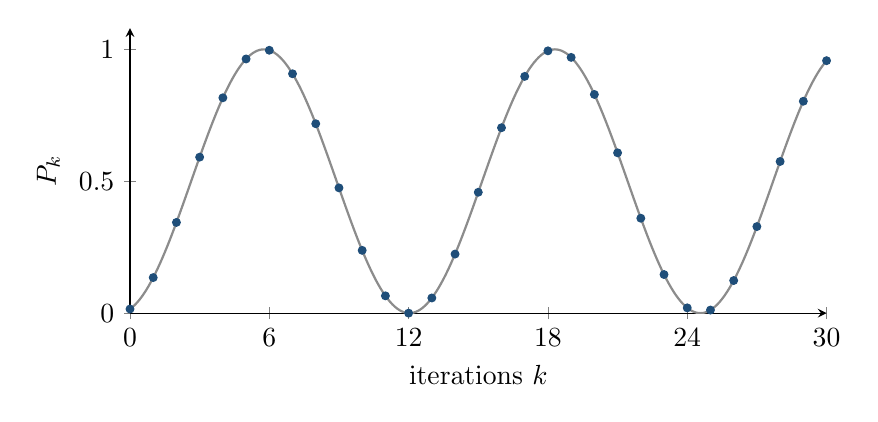
\begin{tikzpicture}
\begin{axis}[width=0.86\linewidth, height=5.2cm, xlabel={iterations $k$}, ylabel={$P_k$}, xmin=0, xmax=30, ymin=0, ymax=1.08,
  axis lines=left, samples=301, domain=0:30, ytick={0,0.5,1}, xtick={0,6,12,18,24,30}]
\addplot[black!45, thick] {(sin(deg((2*x+1)*0.12533)))^2};
\addplot[only marks, mark=*, mark size=1.4pt, brand, samples at={0,1,...,30}] {(sin(deg((2*x+1)*0.12533)))^2};
\end{axis}
\end{tikzpicture}\\
{\small $P_k$ for $n = 6$, one marked item: first peak at $k = 6$, nearly zero near $k = 12$ to $13$, and then a second rise. The notebook measures this same shape in its own Section~9.}
\end{keepfig}

\begin{keyres}{Over-rotation}
More iterations are not better. Past $\kopt$ the state rotates beyond $\ket{m}$ and $P_k$ falls. At $k \approx 2\kopt$ the state is close to $\pm\ket{r}$ and the marked item is \emph{less} likely than for a random guess. The curve is periodic: one full period is $\frac{\pi}{2\theta}$ iterations.
\end{keyres}
\begin{wexample}{Size of the speed-up}
$n = 30$: classical average $2^{29} \approx 5.4\times10^8$ queries; Grover $\frac\pi4\cdot2^{15} \approx 25\,736$ iterations; ratio $\frac2\pi\sqrt N \approx 20\,861$. Large, but only quadratic.
\end{wexample}
\begin{wexample}{Shot statistics}
With $P = 0.99$ and $S = 1000$ shots: marked count $= SP = 990$, with standard deviation $\sqrt{SP(1-P)} = \sqrt{9.9} \approx 3.1$. The Poisson rule $\sqrt{990} \approx 31$ is wrong here because $P$ is close to $1$.
All $S$ shots succeed with probability $P^S \approx e^{-S(1-P)}$: for $P = 0.9999$ and $S = 1000$, about $0.905$. A perfect count does not prove $P = 1$.
\end{wexample}

%=====================================================================================================
\section{The Grover circuit}
\subsection{Building it}
\begin{keepfig}
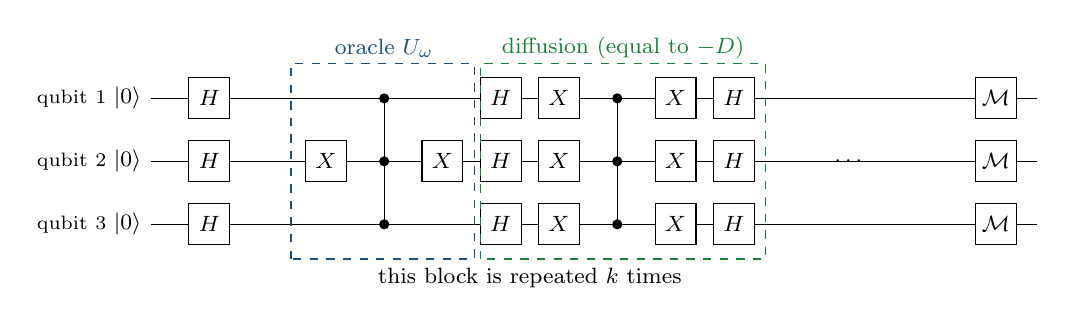
\begin{tikzpicture}[x=0.74cm, y=0.8cm, every node/.style={font=\footnotesize},
  gate/.style={draw, fill=white, minimum size=5.2mm, inner sep=0.5pt}, ctl/.style={circle, fill=black, inner sep=1.3pt}]
  \foreach \y in {0,1,2} {
    \draw (0,\y) -- (15.2,\y);
    \node[left] at (0,\y) {$\ket{0}$};
  }
  \foreach \y in {0,1,2} {
    \node[gate] at (1,\y) {$H$};
    \node[gate] at (6,\y) {$H$}; \node[gate] at (7,\y) {$X$};
    \node[gate] at (9,\y) {$X$}; \node[gate] at (10,\y) {$H$};
  }
  % oracle for x* = 101: X on qubit 2 (middle wire)
  \node[gate] at (3,1) {$X$}; \node[gate] at (5,1) {$X$};
  \draw (4,0) -- (4,2); \foreach \y in {0,1,2} \node[ctl] at (4,\y) {};
  \draw (8,0) -- (8,2); \foreach \y in {0,1,2} \node[ctl] at (8,\y) {};
  \draw[dashed, brand] (2.4,-0.55) rectangle (5.55,2.55); \node[brand] at (4,2.8) {oracle $U_\omega$};
  \draw[dashed, okgreen] (5.65,-0.55) rectangle (10.55,2.55); \node[okgreen] at (8.1,2.8) {diffusion (equal to $-D$)};
  \node at (12,1) {$\cdots$};
  \node at (6.5,-0.85) {this block is repeated $k$ times};
  \foreach \y in {0,1,2} \node[gate] at (14.5,\y) {$\mathcal{M}$};
  \node[left, font=\scriptsize] at (-0.6,2) {qubit 1};
  \node[left, font=\scriptsize] at (-0.6,1) {qubit 2};
  \node[left, font=\scriptsize] at (-0.6,0) {qubit 3};
\end{tikzpicture}\\
{\small Grover circuit for $n = 3$, $\ket{\xs} = \ket{101}$. A column of three dots is the multi-controlled $Z$ (symmetric, so no target is drawn).}
\end{keepfig}

\begin{method}{Oracle for one marked string}
Put $X$ on every qubit where $\xs$ has a $0$, apply the multi-controlled $Z$, and repeat the same $X$ gates. \emph{Example:} $\xs = 0110$ uses $X$ on qubits 1 and 4.
\end{method}

\subsection{The diffusion circuit is $-D$}
Step by step, using the rule for moving a reflection with a unitary:
\[ \mathrm{C}^{n-1}\mathrm{Z} = I - 2\proj{1\dots1} \;\xrightarrow{\;X^{\otimes n}\;}\; I - 2\proj{0\dots0} \;\xrightarrow{\;H^{\otimes n}\;}\; I - 2\proj{s} = -D. \]
The factor $-1$ is a global phase, so the circuit is correct. The notebook's kernel has the same remark in its code comment.

\subsection{Counting gates}
\begin{keyres}{Gates per iteration}
With $z$ the number of $0$s in $\xs$: oracle $= 2z + 1$; diffusion $= 4n + 1$; so \quad total $= 4n + 2z + 2$. \\
Whole circuit: $n + k(4n + 2z + 2)$ gates, plus $n$ measurements.
\end{keyres}
\begin{wexample}{Two counts}
\begin{steps}
\item $n = 5$, $\xs = 10010$: $z = 3$, so $20 + 6 + 2 = 28$ gates per iteration.
\item $n = 4$, $\xs = 1011$, $k = \kopt = 3$: $z = 1$, $16 + 2 + 2 = 20$ per iteration; total $4 + 3\cdot20 = 64$ gates.
\end{steps}
\end{wexample}

\subsection{Cost of a multi-controlled gate}
A multi-controlled $Z$ with $m$ controls can be built with $m - 1$ clean ancillas, $2(m - 1)$ Toffoli gates and one CZ. \emph{Example:} $n = 6$ means $m = 5$: $8$ Toffolis per gate, so $16$ per iteration. This is why hardware circuits grow quickly when multi-controlled gates are decomposed.

\subsection{Reading the notebook's numbers}
\texttt{Grover.ipynb} has one marked item, no ancillas, and calls \texttt{z.ctrl} directly. Its output can be decoded with the formulas above.
\begin{itemize}[itemsep=2pt]
\item \textbf{Gate statistics.} \texttt{h} $= n + 2nk$, \texttt{x} $= k(2n + 2z)$, multi-controlled $Z$ $= 2k$. \emph{Example with $n = 10$, $k = 25$, $z = 4$:} $510$, $700$ and $50$.
\item \textbf{Memory.} On the CPU with the sweep on, it estimates $2\times2^n\times16$ bytes, since two states are held at once. \emph{Example:} $n = 20$ gives $32$ MiB.
\item \textbf{Sweep points.} \texttt{stride} $= \lceil\texttt{sweep\_max}/\texttt{SWEEP\_MAX\_POINTS}\rceil$ with $\texttt{sweep\_max} = 2\kopt + 1$, and the number of points is $1 + \lfloor\texttt{sweep\_max}/\texttt{stride}\rfloor$. \emph{Example:} $\kopt = 25$ with $60$ allowed points: $\texttt{sweep\_max} = 51$, stride $1$, and $52$ points.
\end{itemize}

%=====================================================================================================
\section{Several solutions}
Nothing changes except the angle: $\sin\theta = \sqrt{M/N}$, $\;\kopt \approx \frac\pi4\sqrt{N/M}$. The final state is the uniform superposition of the marked items, so measuring returns a uniformly random solution.
\begin{wexample}{$N = 1024$, $M = 4$}
$\sin\theta = \frac{2}{32} = \frac{1}{16}$, $\;\theta = 0.06254$, $\;\frac{\pi}{4\theta} - \frac12 = 12.06$, so $k = 12$. Compared with $M = 1$ (where $k = 25$), the work has halved, because $\sqrt M = 2$.
\end{wexample}
\begin{center}
\renewcommand{\arraystretch}{1.2}
\begin{tabular}{@{}lccl@{}}
\toprule
$M/N$ & $\theta$ & $P_1 = \sin^2 3\theta$ & What happens\\ \midrule
$\frac18$ & $20.7^\circ$ & $\frac{25}{32}$ & normal; one more step gives $0.945$\\
$\frac14$ & $30^\circ$ & $1$ & \textbf{one iteration is exact}\\
$\frac12$ & $45^\circ$ & $\frac12$ & \textbf{flat}: $P_k = \frac12$ for every $k$\\
$\frac34$ & $60^\circ$ & $0$ & \textbf{worst case}: one iteration erases all marked weight\\
\bottomrule
\end{tabular}
\end{center}
\begin{trap}
When $M > N/2$ do not iterate: measuring immediately succeeds with probability $M/N > \frac12$. Iterating can make things much worse. The formula for $\kopt$ agrees: for $M > N/2$ we have $\theta > \frac\pi4$, so $\frac{\pi}{4\theta} - \frac12 < \frac12$ and it rounds to $0$.
\end{trap}

%=====================================================================================================
\section{Unknown $M$, exact search and fixed-point search}
\subsection{Unknown $M$ (BBHT)}
Choosing $k$ needs $\theta$, hence $M$. Boyer, Brassard, H{\o}yer and Tapp avoid this with randomness.
\begin{keyres}{Average over a random $k$}
\[ \frac1m\sum_{k=0}^{m-1}\sin^2\big((2k+1)\theta\big) = \frac12 - \frac{\sin4m\theta}{4m\sin2\theta}, \]
which is at least $\frac14$ as soon as $m \ge \frac{1}{\sin2\theta} \approx \frac12\sqrt{N/M}$.
\end{keyres}
\begin{method}{BBHT}
(1) Set $m = 1$. (2) Choose $k$ uniformly from $\{0, \dots, \lceil m\rceil - 1\}$ and run $k$ iterations. (3) Measure and test the result with the oracle; stop on success. (4) Otherwise set $m \leftarrow \min(\lambda m, \sqrt N)$ with $\lambda$ such as $\frac65$, and return to (2). The expected number of queries is $O(\sqrt{N/M})$.
\end{method}
\emph{Example:} $n = 10$, $M = 1$: threshold $\approx \frac12\sqrt{1024} = 16$.

\subsection{Exact search}
If $(2k+1)\theta$ misses $\frac\pi2$, shrink the angle a little: use $k = \lceil\frac{\pi}{4\theta} - \frac12\rceil$ and $\theta' = \frac{\pi}{2(2k+1)} \le \theta$. A smaller marked weight (for example from an extra ancilla rotation) gives $P = 1$.
\emph{Example:} $N = 8$: $\theta = 0.3614$, ceiling of $1.67$ is $k = 2$, and $\theta' = \frac{\pi}{10} = 0.3142 < \theta$. \checkmark\ You must round \emph{up}: rounding down needs a larger angle, which reducing the marked weight cannot provide.

\subsection{Fixed-point search}
Grover's $\pi/3$ method replaces the sign flips by phases $\frac\pi3$. One recursion step maps the failure probability $\varepsilon \mapsto \varepsilon^3$, so $\varepsilon_j = \varepsilon^{3^j}$; extra steps cannot over-rotate. \emph{Example:} $\varepsilon = 0.2 \to 0.008 \to 5.12\times10^{-7}$. The basic form gives up the quadratic speed-up; later variants recover it.

\subsection{Maximum success is not minimum cost}
If you repeat until success, with a free check of each result, the expected cost is $k/P_k$ queries.
\begin{wexample}{$N = 16$}
$P_1 = 0.473$, $P_2 = 0.908$, $P_3 = 0.961$. Expected cost: $k/P_k = 2.12$, $2.20$, $3.12$. So $k = 1$ is cheapest, even though $\kopt = 3$. If each check costs one extra query the cost becomes $(k+1)/P_k = 4.23$, $3.30$, $4.16$, and $k = 2$ wins. Read the question to see which is asked.
\end{wexample}

%=====================================================================================================
\section{Amplitude amplification and quantum counting}
\subsection{Amplitude amplification}
Replace $H^{\otimes n}$ by any procedure $\mathcal{A}$ (no measurement) with success probability $a$:
\begin{keyres}{Amplification}
$Q = -\mathcal{A}S_0\mathcal{A}^{-1}S_\chi$, with $S_\chi$ flipping the sign of good states and $S_0 = I - 2\proj{0}$. With $\sin^2\theta = a$:
$P_k = \sin^2((2k+1)\theta)$, using $\mathcal{A}$ or $\mathcal{A}^{-1}$ in total $\mathbf{2k + 1}$ times. Grover is the case $\mathcal{A} = H^{\otimes n}$, $a = M/N$.
\end{keyres}
\begin{wexample}{$a = 0.04$}
$\theta = \arcsin0.2 = 0.2014$, $\;\frac{\pi}{4\theta} - \frac12 = 3.40$, so $k = 3$; $7$ uses of $\mathcal{A}$; $P = \sin^2 7\theta = 0.974$. Classical repetition needs $1/a = 25$ runs on average.
\end{wexample}

\subsection{Eigenstructure of $G$}
Since $G$ is a rotation by $2\theta$ on the plane (Section~2), its eigenvalues there are $e^{\pm2i\theta}$ with eigenvectors $\frac{1}{\sqrt2}(\ket{r} \mp i\ket{m})$. The start state $\ket{s}$ is an equal-weight superposition of the two.

\subsection{Quantum counting}
Apply phase estimation to $G$ with start state $\ket{s}$. Writing the eigenvalue as $e^{2\pi i\varphi}$ gives $\varphi = \frac\theta\pi$ or $1 - \frac\theta\pi$. So outcome $y$ on $t$ counting qubits gives
\[ \tilde\theta = \frac{\pi y}{2^t}, \qquad \tilde M = N\sin^2\tilde\theta. \]
Outcomes $y$ and $2^t - y$ give the same $\tilde M$.
\begin{wexample}{$N = 32$, $M = 8$, $t = 4$}
\begin{steps}
\item $\sin^2\theta = \frac14$, $\theta = \frac\pi6$, so $\varphi = \frac16$ and $\frac56$.
\item On the grid: $16\cdot\frac16 = 2.67$ and $16\cdot\frac56 = 13.33$, so the likely outcomes are $y = 3$ and $y = 13$.
\item From $y = 3$: $\tilde M = 32\sin^2\frac{3\pi}{16} = 32\times0.3087 \approx 9.9$. The true value is $8$: the estimate improves with every extra counting qubit.
\end{steps}
\end{wexample}
\begin{trap}
The eigenphase is $\theta/\pi$, not $\theta/(2\pi)$: the eigenvalue is $e^{2i\theta}$, so $2\pi\varphi = 2\theta$.
\end{trap}

%=====================================================================================================
\section{Limits and applications}
\begin{keyres}{Optimality}
Every quantum algorithm with black-box access needs $\Omega(\sqrt{N/M})$ queries (Bennett, Bernstein, Brassard, Vazirani). Zalka proved that $\frac\pi4\sqrt N$ is optimal for $M = 1$ including the constant. \textbf{Grover cannot be improved in the black-box setting.}
\end{keyres}
\begin{itemize}[itemsep=2pt]
\item \textbf{NP-complete problems:} search over $2^n$ assignments takes about $2^{n/2}$ iterations, which is still exponential. Grover does not make these problems polynomial. For $40$ variables, $\frac\pi4 2^{20} \approx 823\,550$ iterations.
\item \textbf{Parallel search:} $p$ machines reduce the time by only $\sqrt p$, and the total queries increase by $\sqrt p$. Four machines: half the time, twice the queries. Classically, the time falls by $p$ with constant total work.
\item \textbf{Keys:} a $k$-bit key needs about $2^{k/2}$ iterations, and each one must run the cipher reversibly. Doubling the key length restores the margin: AES-256 still has about $2^{128}$ iterations.
\item \textbf{Noise:} in a simple model, $P_k \approx f^{k}\sin^2((2k+1)\theta) + (1 - f^k)/N$. For $f = 0.995$, $k = 25$: $f^k \approx 0.88$. Because $k \propto \sqrt N$, large searches need very low error rates.
\item \textbf{Simulation:} state-vector work grows like $k\cdot2^n \sim 2^{1.5n}$, a factor of $2\sqrt2$ per qubit. The notebook's $n = 15$ default takes about a minute including its sweep.
\end{itemize}
\begin{center}
\renewcommand{\arraystretch}{1.2}
\begin{tabularx}{\linewidth}{@{}lcX@{}}
\toprule
\textbf{Task} & \textbf{Queries} & \textbf{Comment}\\ \midrule
Unstructured search, classical & $\Theta(N)$ & must check a constant fraction of items\\
Unstructured search, quantum & $\Theta(\sqrt N)$ & Grover; optimal\\
Collision in a 2-to-1 function & $\Theta(N^{1/3})$ & Brassard--H{\o}yer--Tapp; lower bound by Aaronson--Shi\\
Element distinctness & $\Theta(N^{2/3})$ & Ambainis's quantum walk\\
\bottomrule
\end{tabularx}
\end{center}
Other uses include minimum finding (D{\"u}rr--H{\o}yer) and speeding up the classical part of many algorithms by amplitude amplification.

%=====================================================================================================
\section{Problem-solving strategies}
\subsection{Strategy by question format}
\begin{itemize}[itemsep=3pt]
\item \textbf{Single-correct numerical:} compute fully, then sanity-check (probabilities in $[0,1]$; $\sum|c_x|^2 = 1$; compare inversion about the mean with $\sin^2((2k+1)\theta)$). Many distractors are ``forgot to square'', ``used $\sqrt N$ without $\frac\pi4$'', ``dropped the $-\frac12$'', ``used the mean instead of the new amplitude''.
\item \textbf{Matching lists:} solve the easiest row first; often one row fixes the option.
\item \textbf{Assertion--Reason:} decide A and R \emph{independently} first. Only if both are true ask: does R \emph{cause} A?
\item \textbf{Statement I/II:} judge each statement alone; one counterexample kills ``never'' or ``always'' ($N = 4$, $k = 2$ is a useful one).
\item \textbf{Paragraph:} the first question usually sets up a quantity reused in the second; write it down clearly.
\end{itemize}

\subsection{Fast checks that catch most mistakes}
\begin{enumerate}[itemsep=2pt]
\item Is the state still normalised after your step?
\item Is $M/N$ a special ratio ($\frac14, \frac12, \frac34$)?
\item Compute $P_k$ both ways: amplitudes and $\sin^2((2k+1)\theta)$.
\item Is $k$ past $\kopt$? Then expect over-rotation.
\item Does the $X$ pattern match the \emph{zeros} of $\xs$?
\end{enumerate}

\subsection{Map: assessment questions $\to$ sections of this chapter}
\begin{tabularx}{\linewidth}{@{}lX@{}}
\toprule
\textbf{Questions} & \textbf{Where to learn it}\\ \midrule
Q.1, Q.5, Q.15, Q.17, Q.19, Q.20 & Section 1 (phases, identities, the $\sin^2$ curve, peak and period)\\
Q.2--Q.4, Q.16, Q.18, Q.30 & Section 2 (reflections, rotations, eigenvalues, traces)\\
Q.7--Q.11, Q.13 & Section 3 (inversion about the mean, counting, classical search, scaling)\\
Q.12, Q.14, Q.21, Q.22, Q.28, Q.29, Q.31, Q.32, Q.38 & Section 4 (normalisation, tensor products, Born rule, phases, subspace measurement, overlaps, memory)\\
Q.23--Q.27, Q.33, Q.35, Q.36, Q.39, Q.40 & Section 5 (Hadamard layers, $X$ conjugation, kickback, entanglement)\\
Q.37, Q.57 & Section 6 (what the oracle does and does not do)\\
Q.34, Q.41, Q.42, Q.44, Q.48, Q.59, Q.60 & Section 7 (the matrix of $D$, tracing amplitudes by hand)\\
Q.6, Q.43, Q.52--Q.55, Q.58, Q.73 & Section 9 (optimal $k$, over-rotation, speed-up, shots)\\
Q.45--Q.47, Q.56, Q.65, Q.67, Q.70, Q.72 & Section 10 (circuit, $-D$, gate counts, reading the notebook's numbers)\\
Q.49--Q.51, Q.61, Q.78 & Section 11 (several solutions, special ratios)\\
Q.62, Q.63, Q.74 & Section 12 (BBHT, exact search, cost)\\
Q.66, Q.76, Q.79, Q.80 & Section 13 (amplification, counting)\\
Q.64, Q.68, Q.69, Q.71, Q.75, Q.77 & Section 14 (optimality, keys, noise, simulation, complexity)\\
\bottomrule
\end{tabularx}
{\small (Section 8, the geometric picture, underlies all of Q.41--Q.80.)}

%=====================================================================================================
\section{Practice problems}
Try each before looking at the answers on the next page. They use the same ideas as the assessment but different numbers.
\begin{enumerate}[label=\textbf{P\arabic*.}, leftmargin=2.6em, itemsep=1pt]
\item Let $\sin\theta = \frac15$. Find $\sin^2 3\theta$ exactly.
\item Find $2uu^{T} - I$ for $u = \frac{1}{\sqrt2}(1, 1)^{T}$.
\item Lines at $15^\circ$ and $75^\circ$: reflect in the first, then in the second. What is the combined map?
\item $v = (1, 1, 1, -1)$. Find the result of inversion about the mean.
\item $N = 15$ items, $M = 4$ marked. Expected draws without replacement until the first marked one?
\item $f = x_1 \land (x_2 \lor x_3)$ on three bits. Find $M/N$.
\item $\ket\psi = \frac{1}{\sqrt6}(\ket{00} + \ket{01} - 2\ket{11})$. Find $P(\text{the bits are equal})$ and the state afterwards.
\item Which basis state has its sign flipped by $X_1X_3\,\mathrm{CCZ}\,X_1X_3$?
\item Is $\frac12(\ket{00} - \ket{01} - \ket{10} - \ket{11})$ entangled?
\item $N = 64$, one marked item, one iteration: find the marked amplitude (in units of $a = 1/8$) and $P_1$.
\item Find $\kopt$ for $n = 12$, one marked item ($\theta \approx 0.015626$).
\item $N = 64$, $M = 16$: find $P_1$.
\item Gates per iteration for $n = 7$, $\xs = 0011010$.
\item $N = 128$, $M = 2$: find $\kopt$.
\item Amplitude amplification with $a = \frac19$ ($\theta \approx 0.3398$): find the optimal $k$, the uses of $\mathcal{A}$, and $P$.
\item Quantum counting with $N = 16$, $M = 4$, $t = 4$: the likely $y$ and the resulting $\tilde M$.
\end{enumerate}

\newpage
\subsection*{Answers to the practice problems}
\begin{enumerate}[label=\textbf{P\arabic*.}, leftmargin=2.6em, itemsep=3pt]
\item $\sin3\theta = \frac35 - \frac{4}{125} = \frac{71}{125}$; so $\sin^2 3\theta = \frac{5041}{15625}$.
\item $uu^{T} = \frac12\begin{psmallmatrix}1&1\\1&1\end{psmallmatrix}$, so $2uu^{T} - I = \begin{psmallmatrix}0&1\\1&0\end{psmallmatrix} = X$.
\item Rotation by $+120^\circ$.
\item Mean $\frac12$; result $(0, 0, 0, 2)$. Length check: $4 = 4$.
\item $\frac{16}{5} = 3.2$.
\item $x_1 = 1$ and $3$ of the $4$ pairs $(x_2, x_3)$: $M = 3$, so $\frac38$.
\item $P = \frac{1 + 4}{6} = \frac56$; new state $\frac{\ket{00} - 2\ket{11}}{\sqrt5}$.
\item $\ket{010}$.
\item $c_{00}c_{11} = -\frac14$ and $c_{01}c_{10} = \frac14$: entangled.
\item Mean $\frac{62}{64}a = \frac{31}{32}a$; marked $\frac{31}{16}a + a = \frac{47}{16}a$; $\;P_1 = \frac{2209}{256}\cdot\frac{1}{64} = \frac{2209}{16384} \approx 0.135$.
\item $\frac{\pi}{4\theta} - \frac12 = 50.26 - 0.5 = 49.76$, so $\kopt = 50$.
\item $M/N = \frac14$, so $\theta = 30^\circ$ and $P_1 = 1$.
\item $z = 4$: $4\cdot7 + 8 + 2 = 38$.
\item $\sin\theta = \frac18$, $\theta = 0.12533$, $\frac{\pi}{4\theta} - \frac12 = 5.77$: $\kopt = 6$.
\item $\frac{\pi}{4\theta} - \frac12 = 1.81$: $k = 2$; $5$ uses; $P = \sin^2 5\theta \approx 0.983$.
\item $\theta = \frac\pi6$, $\varphi = \frac16, \frac56$; $y \approx 2.67$ and $13.33$, so $y = 3$ or $13$; $\tilde M = 16\sin^2\frac{3\pi}{16} \approx 4.9$.
\end{enumerate}

\subsection*{Summary of the chapter in ten lines}
\begin{enumerate}[itemsep=1pt]
\item Classical search costs about $N/M$ queries; Grover costs about $\frac\pi4\sqrt{N/M}$ iterations.
\item Oracle $U_\omega$ flips the sign of marked items: invisible until interference follows.
\item Diffusion $D = 2\proj{s} - I$ is inversion about the mean: $c_x \mapsto 2\bar c - c_x$.
\item Circuit: $X$ on the zeros of $\xs$, multi-controlled $Z$, $X$ again; then $H$, $X$, multi-controlled $Z$, $X$, $H$ (which is $-D$).
\item Two reflections are a rotation by twice the angle between them: $G$ rotates by $2\theta$.
\item $\sin\theta = \sqrt{M/N}$; $\;P_k = \sin^2((2k+1)\theta)$; $\;\kopt = \operatorname{round}(\frac{\pi}{4\theta} - \frac12)$.
\item More iterations over-rotate: $P_k$ oscillates. $M = \frac N4$ is exact, $\frac N2$ is flat, $\frac{3N}{4}$ is the worst case for one iteration.
\item Unknown $M$: BBHT. Exact: shrink the angle. No over-rotation: fixed-point search.
\item Amplitude amplification: $\mathcal{A}$ with success $a$, $2k + 1$ uses. Counting: phase estimation of $G$, whose eigenvalues are $e^{\pm2i\theta}$.
\item $\Omega(\sqrt N)$ is a proven lower bound: the speed-up is quadratic, never exponential.
\end{enumerate}
\end{document}
